%%
% The BIThesis Template for experiment report
%
% Copyright 2020 Spencer Woo, Silvester Wang
%
% Compile with: xelatex -> xelatex -> xelatex

\documentclass[UTF8,AutoFakeBold,AutoFakeSlant,12pt]{ctexart}
\usepackage[a4paper,left=3.18cm,right=3.18cm,top=2.54cm,bottom=2.54cm,includeheadfoot]{geometry}
\usepackage{fontspec}
\usepackage{setspace}
\usepackage{graphicx}
\usepackage{fancyhdr}
\usepackage{titlesec}
\usepackage{pdfpages}
\usepackage{setspace}
\usepackage{booktabs}
\usepackage{multirow}
\usepackage{float}
\usepackage{caption}


% 将你的相关信息替换如下示例
\newcommand{\reportName}{通信课程实验报告}
\newcommand{\deptName}{计算机学院}
\newcommand{\majorName}{计算机科学与技术}
\newcommand{\className}{07xxxxxx}
\newcommand{\yourName}{惠计算}
\newcommand{\teacherName}{张哈希}

% 定义一个概念
% \newtheorem{definition}{概念}[section]

% 将西文字体设置为 Times New Roman
\setromanfont{Times New Roman}

% 设置引用位于右上角
\newcommand{\upcite}[1]{\textsuperscript{\cite{#1}}}

% 设置文档标题深度
\setcounter{tocdepth}{3}
\setcounter{secnumdepth}{3}

%%
% 设置一级标题、二级标题格式
\ctexset{section={
  format={\raggedright \bfseries \songti \zihao{-3}},
  name = {,.},
  number = \chinese{section}
  }
}
\ctexset{subsection={
  format = {\bfseries \songti \raggedright \zihao{-4}},
  }
}

\begin{document}

\begin{titlepage}
  \centering

  \vspace{23mm}

  
\includegraphics[width=.5\textwidth]{assets/logo_bit.png}

  \vspace{10mm}

  \heiti\fontsize{24pt}{24pt}\selectfont{\reportName}

  \vspace{77mm}

  \begin{spacing}{2.2}
    \songti\fontsize{16pt}{16pt}\selectfont{\textbf{学\hspace{11mm}院:}\underline{\makebox[51mm][c]{\deptName}}}

    \songti\fontsize{16pt}{16pt}\selectfont{\textbf{专\hspace{11mm}业:}\underline{\makebox[51mm][c]{\majorName}}}

    \songti\fontsize{16pt}{16pt}\selectfont{\textbf{班\hspace{11mm}级:}\underline{\makebox[51mm][c]{\className}}}

    \songti\fontsize{16pt}{16pt}\selectfont{\textbf{姓\hspace{11mm}名:}\underline{\makebox[51mm][c]{\yourName}}}

    \songti\fontsize{16pt}{16pt}\selectfont{\textbf{任课教师:}\underline{\makebox[51mm][c]{\teacherName}}}
  \end{spacing}

  \vspace{33mm}

  \centering
  \songti\fontsize{12pt}{12pt}\selectfont{\today}
\end{titlepage}


%%
% 正文开始
\pagestyle{fancy}
% 正文从第一页开始计算页码
\setcounter{page}{1}
% 页眉和页脚(页码)的格式设定
\fancyhf{}
\fancyhead[L]{\fontsize{10.5pt}{10.5pt}\selectfont\kaishu{\reportName}}
\fancyfoot[C]{\fontsize{9pt}{9pt}\selectfont\kaishu{\thepage}}
\renewcommand{\headrulewidth}{0.5pt}
\renewcommand{\footrulewidth}{0pt}

\section{实验目的}
\begin{enumerate}
  \item 验证抽样原理
  \item 观察了解 PAM 信号形成过程
  \item 了解混沌效应形成原因
\end{enumerate}

\section{实验仪器}
\begin{enumerate}
  \item ZH7001 通信原理综合实验系统
  \item 20MHz 双踪示波器
  \item 函数信号发生器
\end{enumerate}

\section{实验原理}
利用抽样脉冲把一个连续信号变为离散时间样值的过程称为抽样,抽样后的信号称为脉冲调幅(PAM)信号。抽样定理指出,一个频带受限的信号 $m(t)$,如果他的最高频率为 $f_h$,那么可以唯一的由频率大于或等于 $2f_h$ 的样值序列所决定,即可以由抽样序列无失真地还原原始信号,抽样序列保留原始信号的全部信息。

\section{实验过程}
\subsection{近似理想抽样脉冲序列测量}
函数信号发生器产生正弦信号,频率为 1 KHz,输出电平为 1Vp-p。

波形图如下图\ref{波形图}。

\begin{figure}[H]
  \centering
  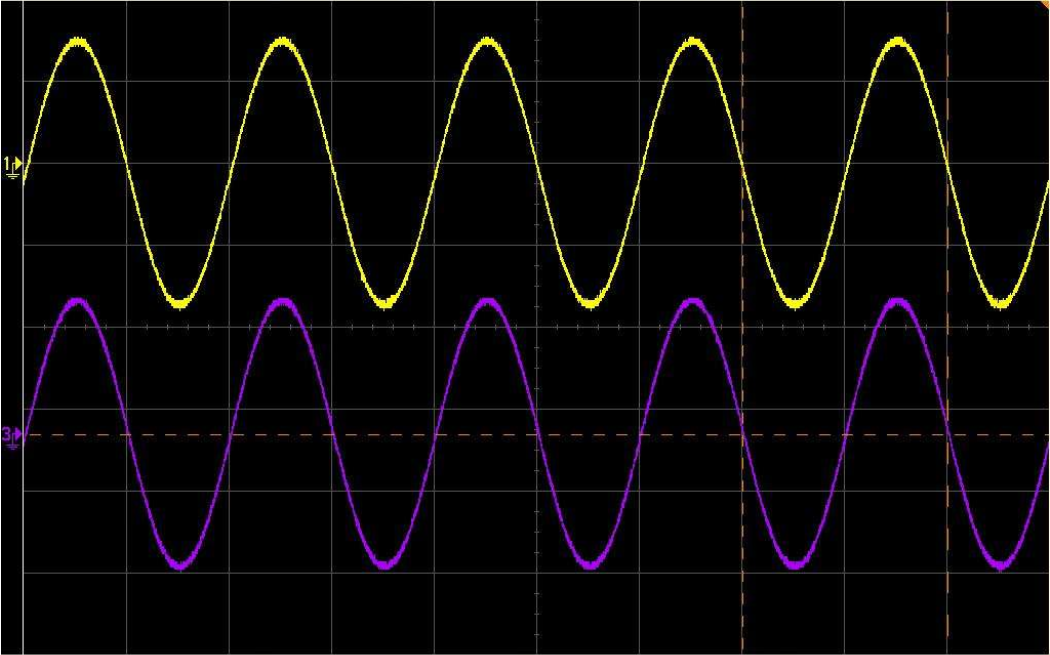
\includegraphics[width=0.63\textwidth]{assets/p1.jpg}
  \caption{波形图}
  \label{波形图}
\end{figure}

\subsection{理想抽样信号重建观察}
理想抽样信号

\section{实验总结}
通过这次实验,我从中知道了抽样原理。

\end{document}
